Here is the application domain model of this project. In particular, this section focuses on the object model (\textbf{static information models} and \textbf{dynamic class behaviour models}).
\subsection{Static Information Model}
The below high-level diagram provides a static information model of the application domain. Basically, it is the structure of the world, it contains only few attributes, and it doesn't include every class that will be necessary to define the model of the CLup system. \newline

The main aspects of Clup modelled in the below diagram are:
\begin{itemize}
    \item The application need to consider the presence of unregistered customers who arrive at the supermarket and require a place in the queue. For this reason, two types of customer (unregistered and registered) are distinguished in the diagram.
    \item Given the need to allow the reservation of a seat in the queue to those who do not use the system directly, it is necessary to distinguish between 2 types of Lineup turn (physical and virtual).
    \item A registered customer can book a Visit or a Lineup turn. To facilitate the reading of the diagram these two actions were generalized to an abstract class Reservation extended by Visit class and LineupTurn class.
    \item An unregistered customer can book only a physical lineup turn. This reservation is handled by a Store employee who will act as a link between the system and the unregistered customer.
    \item Each entrance could be monitored by the store manager.
\end{itemize}
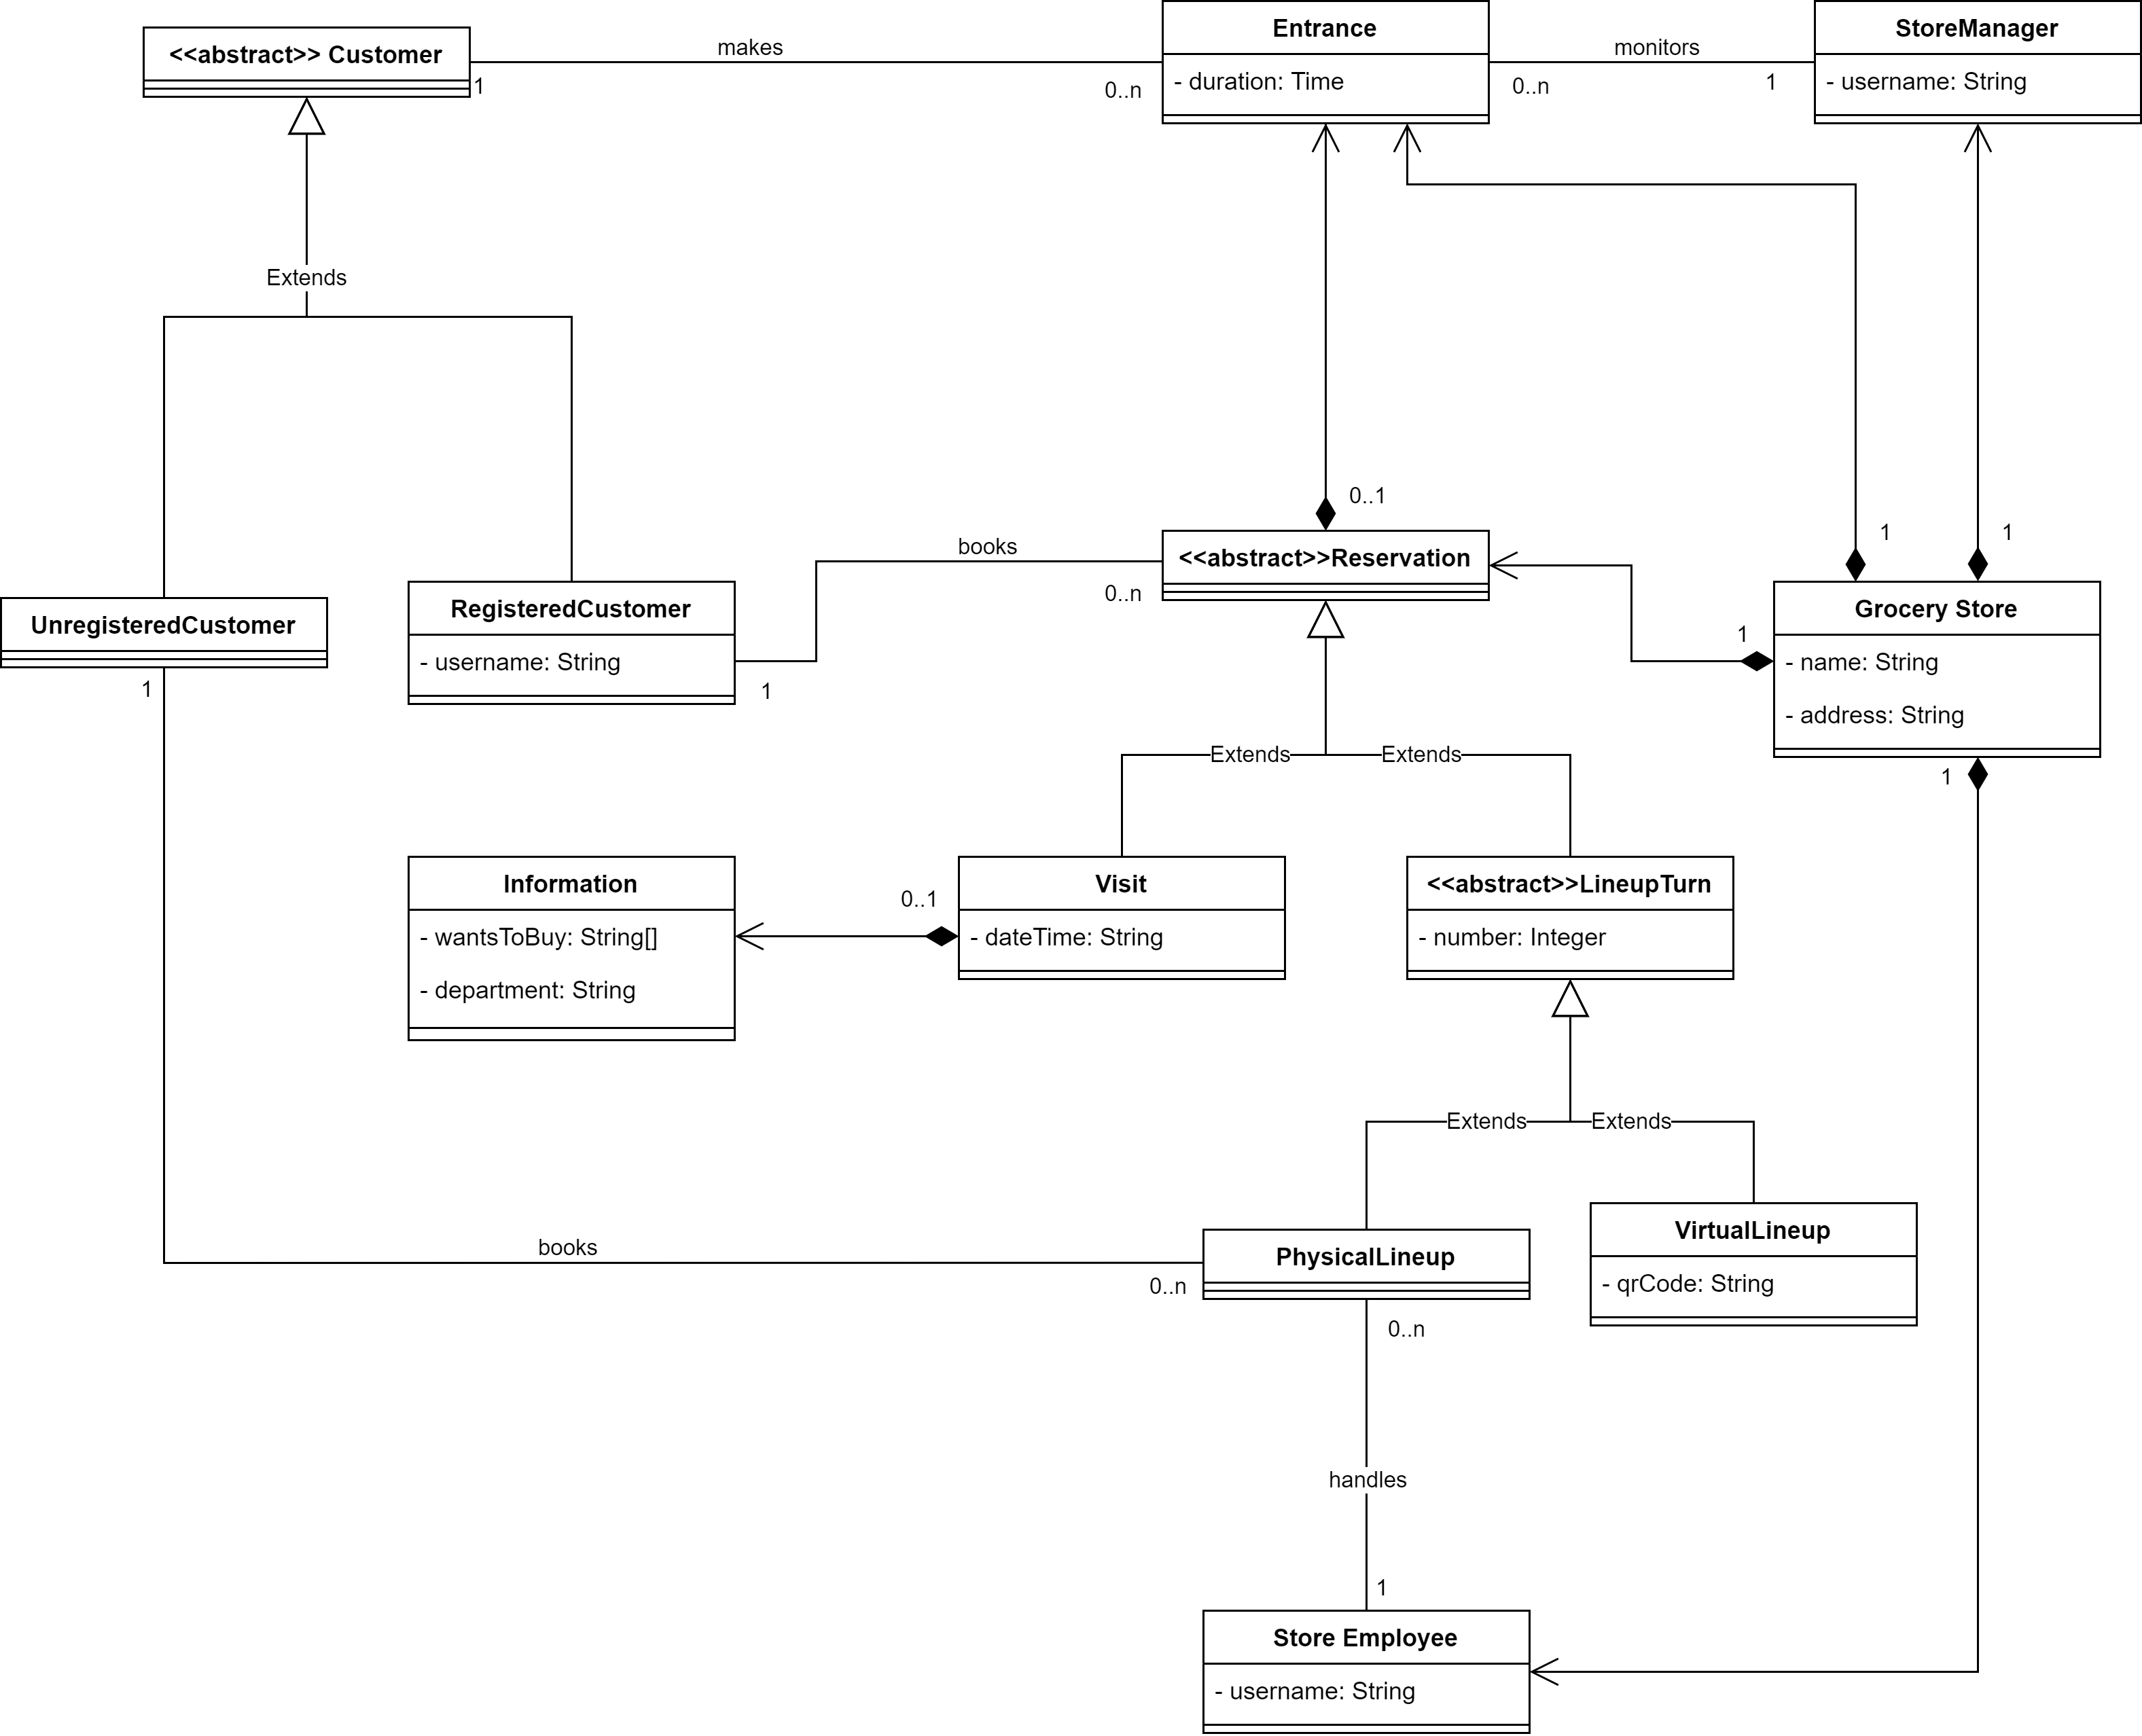
\includegraphics[width=\textwidth]{class_diagram.png}


\subsection{Dynamic Class Behaviour Models}
The below state diagrams shows some	critical aspects of	the	application, how the behaviour of these critical aspects is modeled and the evolution of their states. \newline

In the first state diagram, we model the behavior our system has to have when there is a new request to reserve a virtual lineup turn. Particular attention is paid to the possibility of generating a QR code and the management of waiting in the virtual lineup. \newline


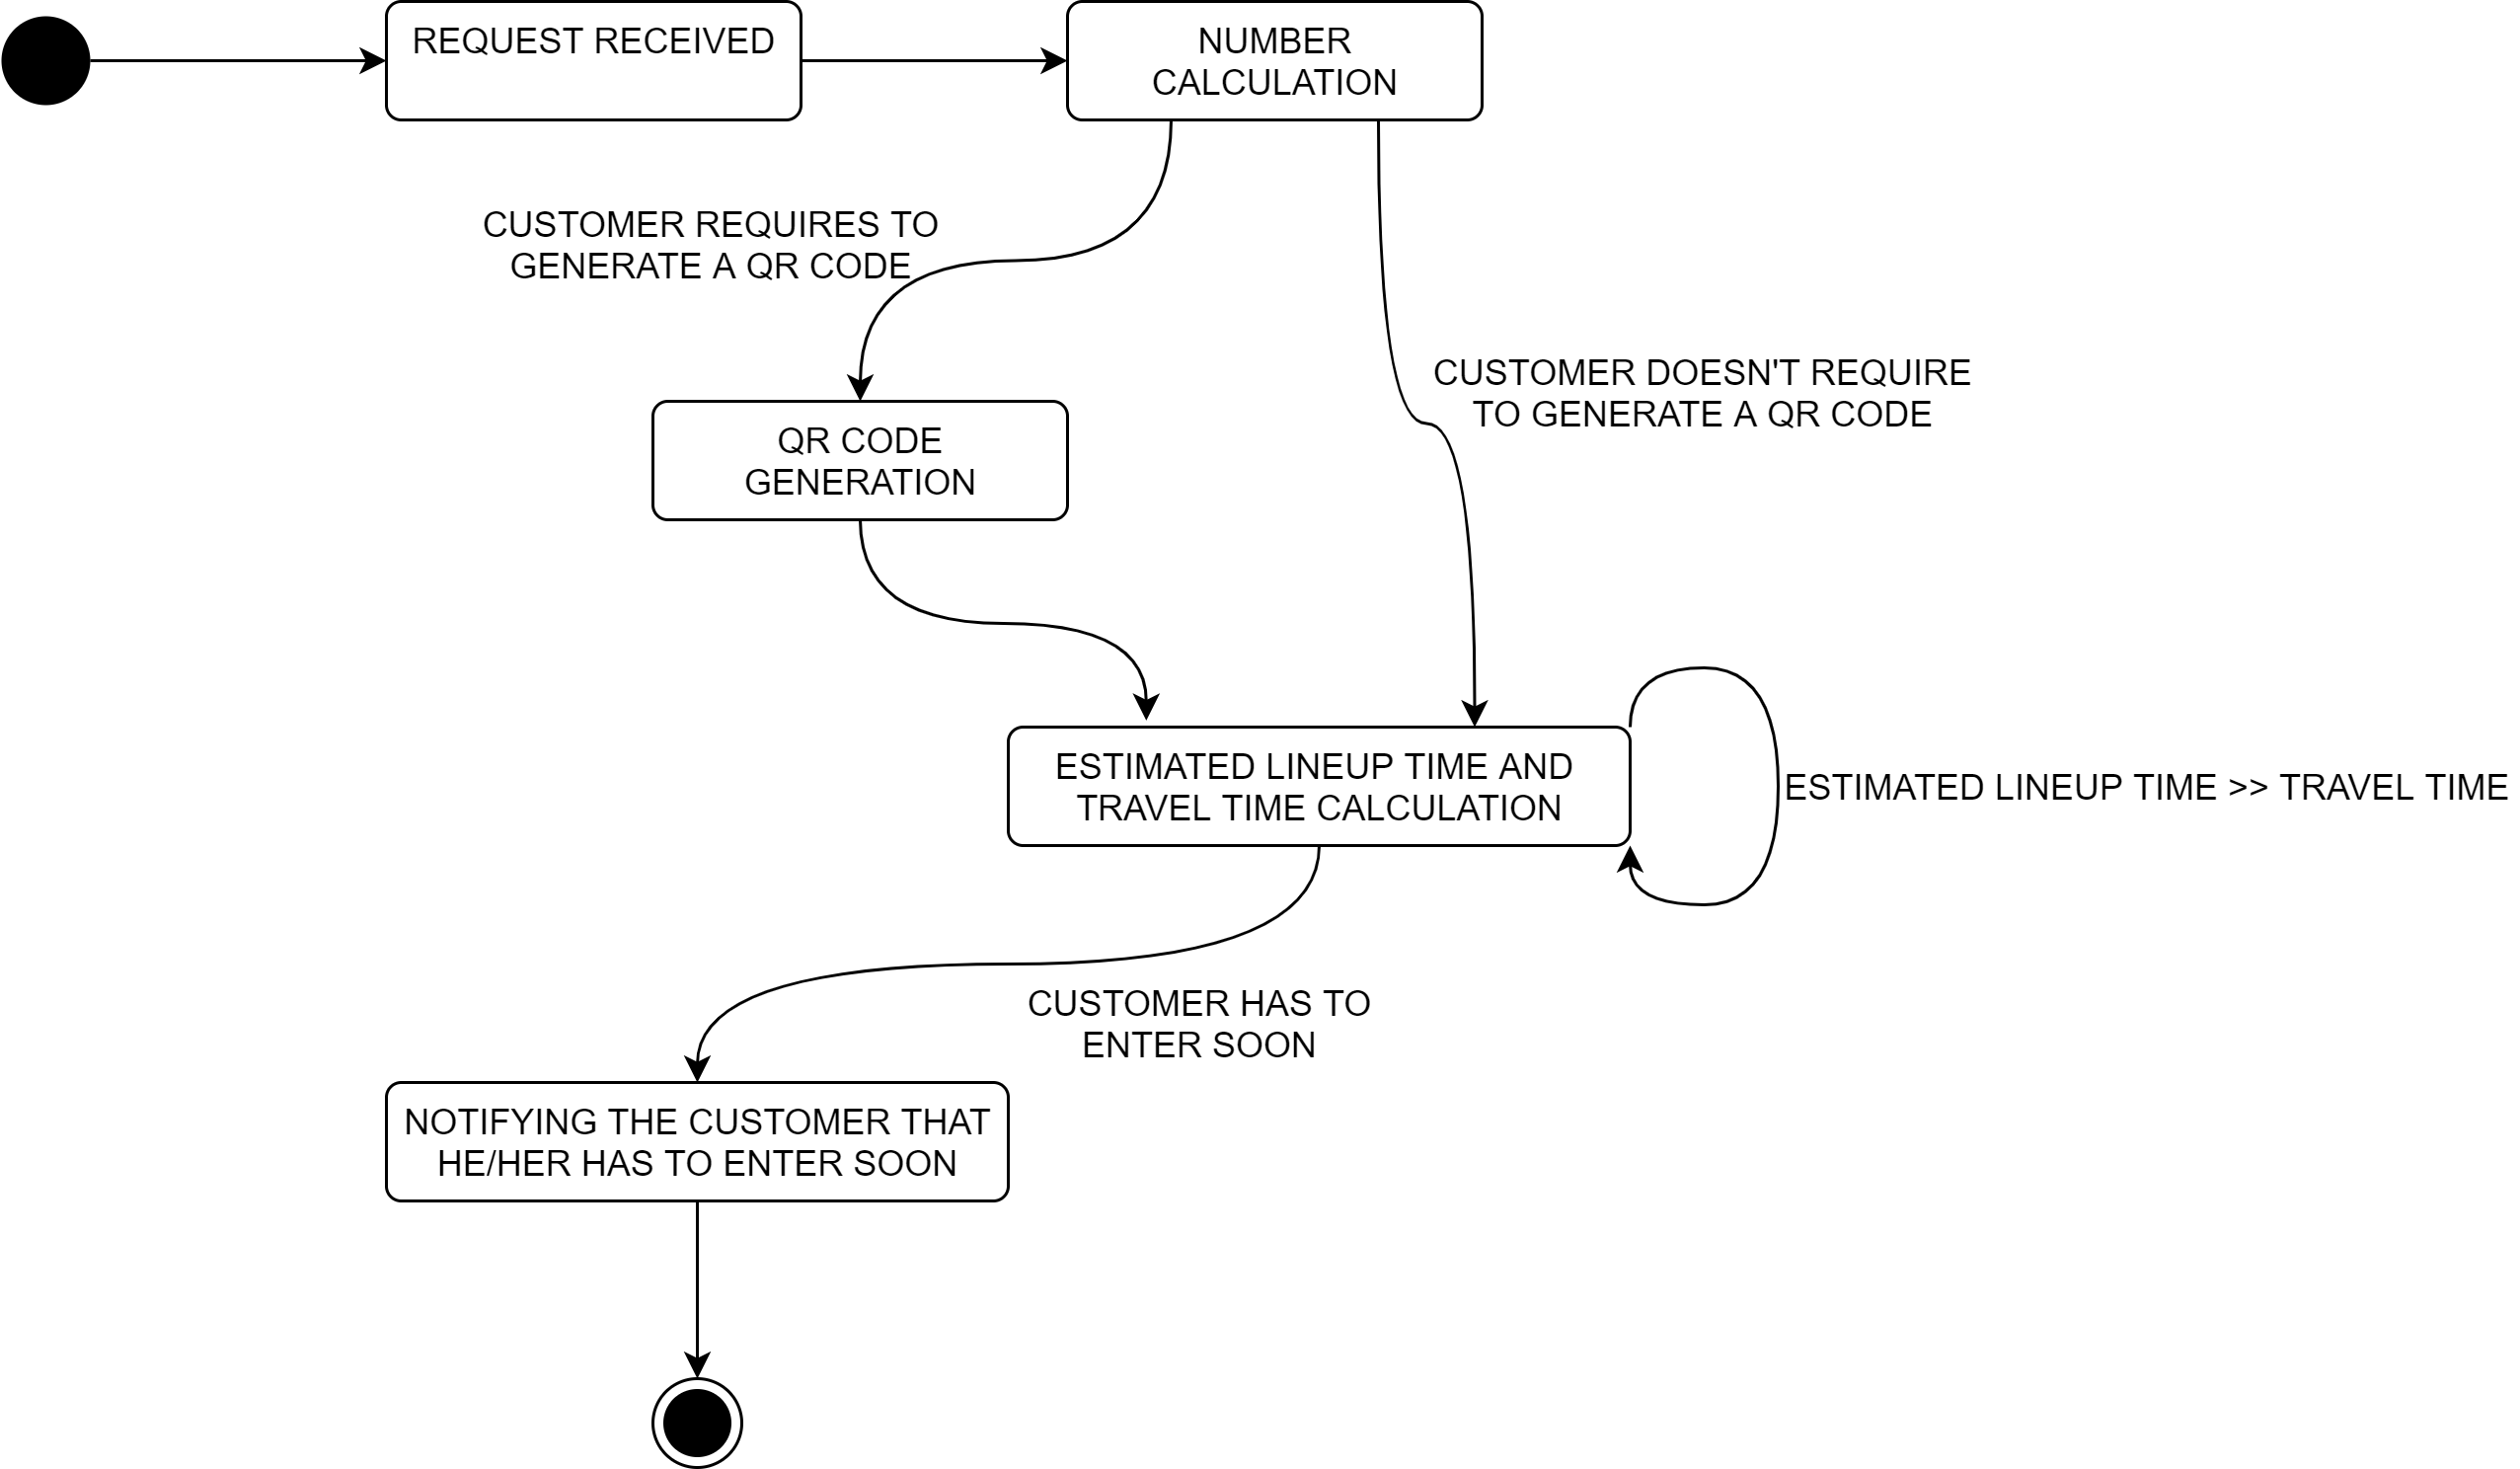
\includegraphics[width=\textwidth]{state_diagram1.png} \newline


In the second state diagram, we model the behavior our system has to have when a store employee notifies a new request to reserve a physical lineup turn. Attention is paid to the difference from the previous phenomenon. In this case, the system will limit itself to acquire the demand and to process it with the other demands (also virtual) \newline


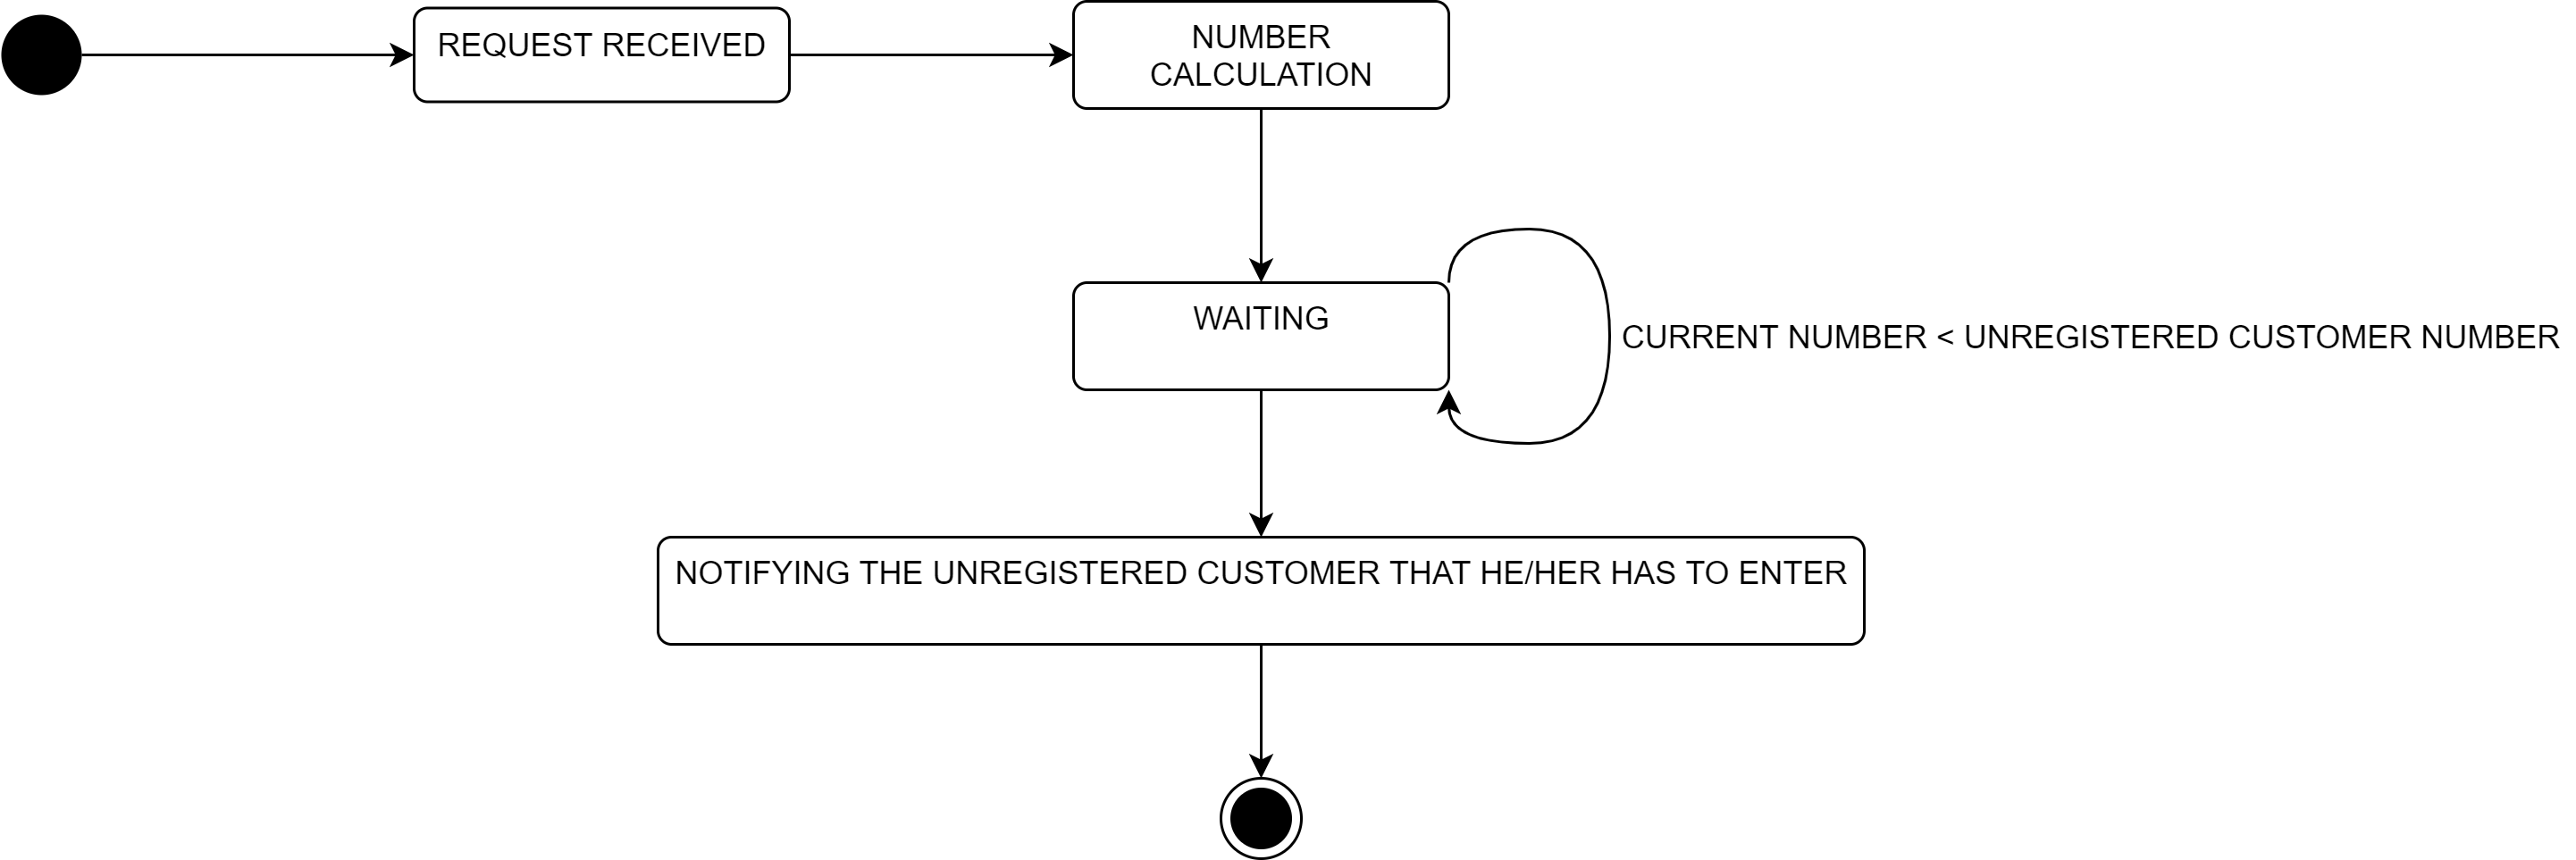
\includegraphics[width=\textwidth]{state_diagram2.png} \newline


In the third and last diagram, we model the behavior our system has to have when there is a new request for booking a visit. Attention is paid to the possibility of following various paths to reach the end of the request. These numerous paths are due to the optional insertion of information related to the visit (department, products to buy, and estimated time). Also, for long-term customers, the estimated time is calculated by the system based on previous entries. \newline 

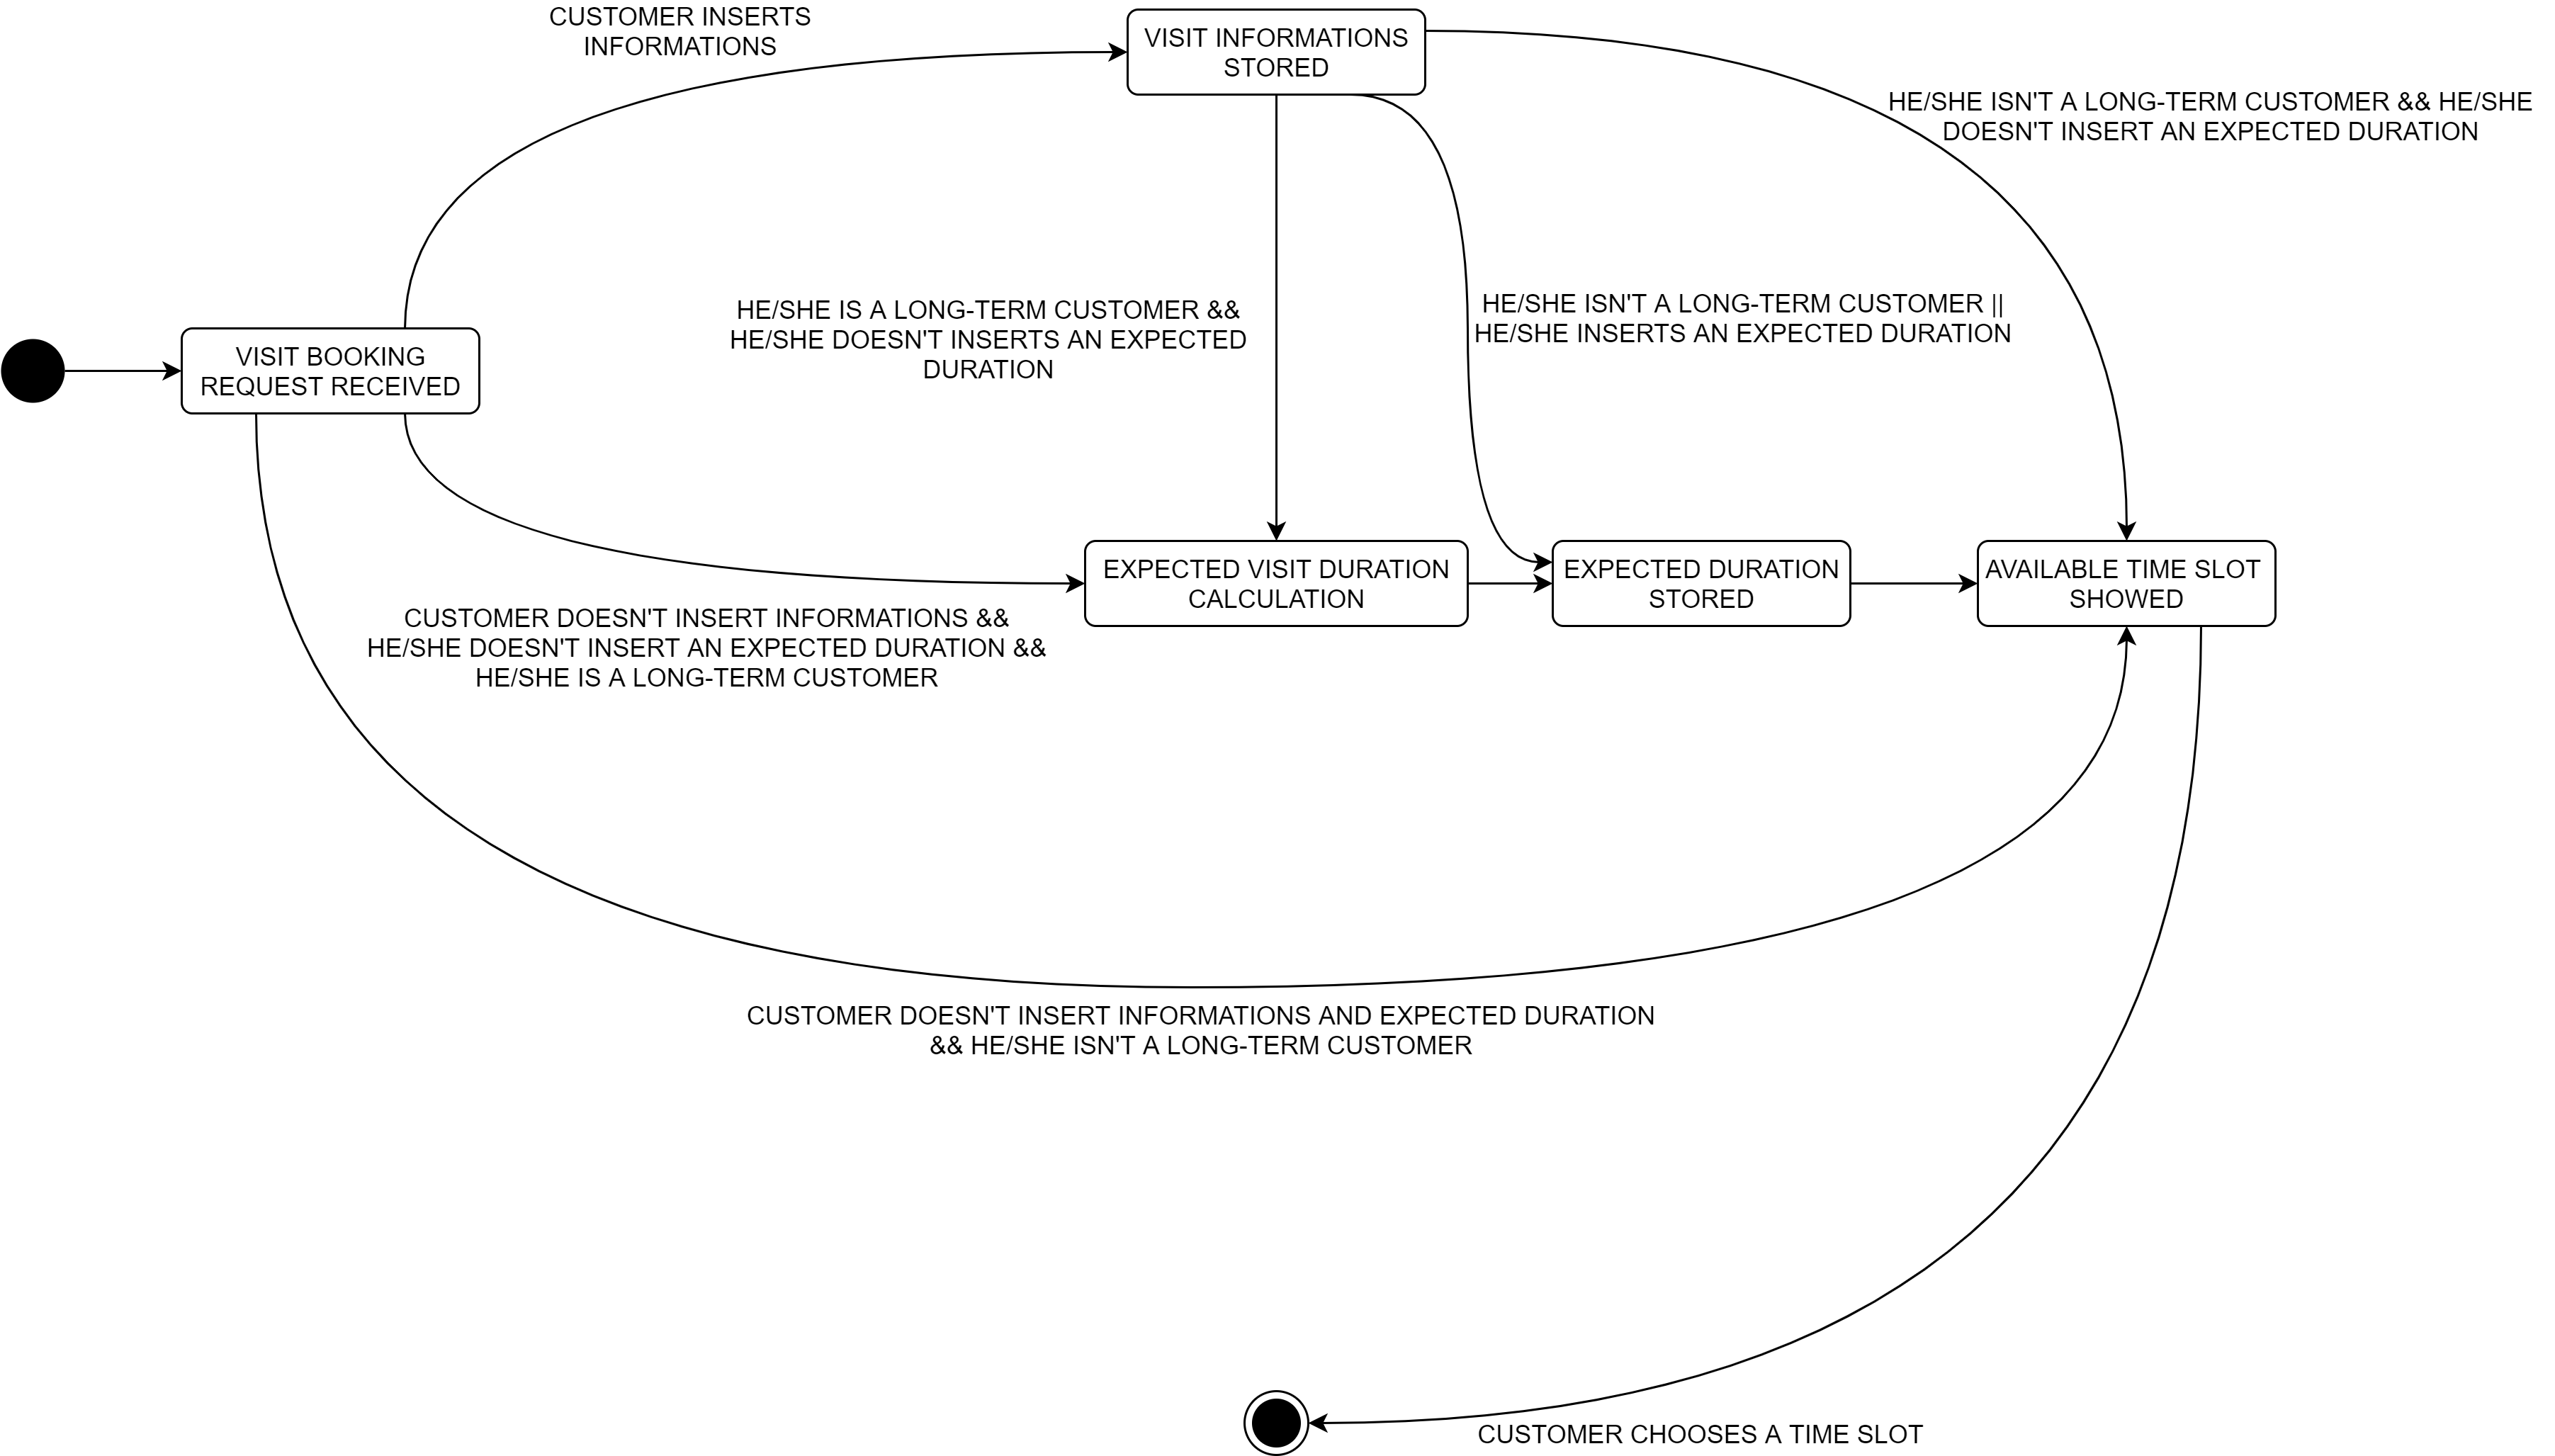
\includegraphics[width=\textwidth]{state_diagram3.png} \newline